Dans cette section, on utilise notre modèle entraîné sur la totalité des données d'entraînement fournies avec l'énoncé et on l'applique sur les données de test non-étiquetées fournies avec l'énoncé. On présente ici les 30 premières prédictions ainsi obtenues.

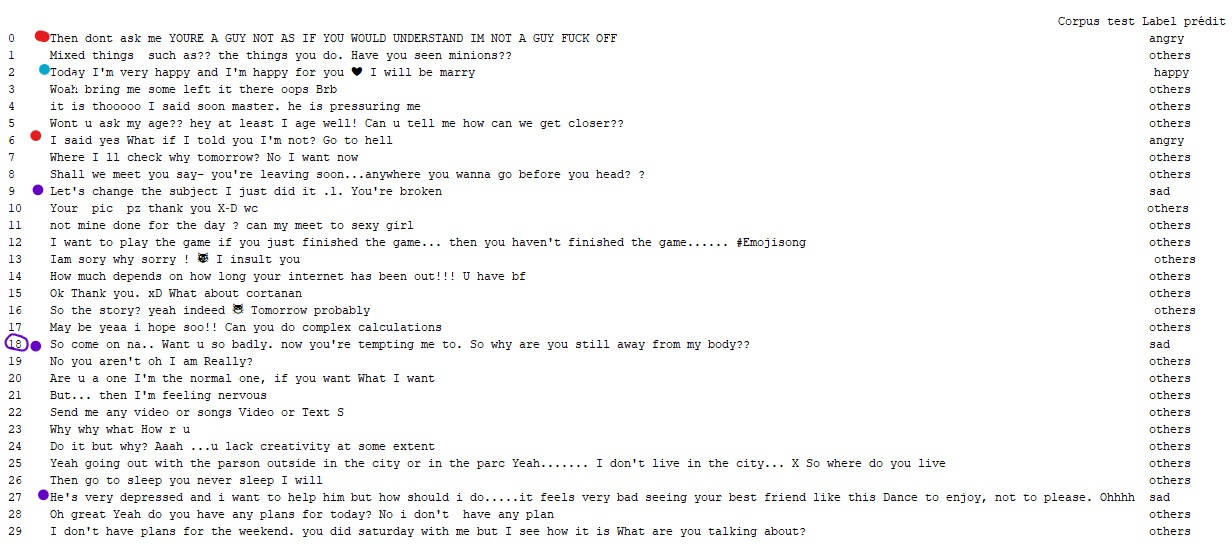
\includegraphics[width=\linewidth,keepaspectratio]{images/couleur_predictions}

Il est difficile d'analyser quantitativement nos prédictions puisque nous n'avons pas les vraies classes associées à chacune des observations de ce corpus.

On peut toutefois voir en regardant l'échantillon de prédictions ci-dessus qu'à chaque fois qu'on prédit happy, angry ou sad, la prédiction semble bonne sauf pour le numéro 18 qui n'a clairement pas l'air triste. On peut supposer que cet échange cocasse est mal classé à cause de "Want u so badly". En effet, le mot \emph{"badly"} a une forte connotation négative, ce qui induit notre modèle à classer ce texte en tant que triste.

En regardant rapidement, on peut voir que ceux classés comme \emph{others} ont l'air particulièrement neutre, sauf peut-être le 13, mais cela est assez subjectif.

Ce petit échantillon nous laisse avec une très bonne impression de notre modèle en prédiction hors-échantillon.